\documentclass[11pt,a4paper]{book}
\usepackage[utf8]{inputenc}
\usepackage[spanish]{babel}
\usepackage{amsmath}
\usepackage{amsfonts}
\usepackage{amssymb}
\usepackage[left=2cm,right=2cm,top=2cm,bottom=2cm]{geometry}
\usepackage{cite}
\author{Víctor de Tejada Molera}

\begin{document}
\chapter{Estado del arte}
    En este capítulo se pretende realizar un análisis del estado del arte referente a los experimentos psicoacústicos; concretamente aquellos que se centran principalmente en la evaluación de diferencias perceptuales en entornos cerrados como auditorios, cines, salas de conferencias, etc.
    
    Para la búsqueda de esta información, se recurre a bases de datos científicas como el sistema \textit{Ingenio UPM} y buscadores de artículos científicos como \textit{Google Scholar}. Con ellos, se han introducido términos de búsqueda como ``\textit{Psychoacoustics}'', ``\textit{Subjective test acoustics}'' o ``\textit{Auditorium subjective test}''. Los resultados arrojados por dichas plataformas, se revisan y se lee el resumen o \textit{abstract} de los que se consideran que pueden ser útiles para el proyecto. Si el resumen confirma que la temática concuerda con la del estudio, se procede a la lectura del resto del artículo y se extraen los elementos que se consideran más importantes. Estos son principalmente: el tipo de análisis estadístico que se ha utilizado, el número de personas que han realizado el test, el tipo de test (tipo de preguntas, formato, duración de los audios utilizados, etc.), entre otros.
    
    Por otro lado, se ha realizado, paralelamente, una búsqueda de fuentes bibliográficas especializados en temas como de detección de señales, análisis estadístico de datos y, más específicamente, sobre modelos Thurstonianos. Para ello, se realizan nuevas consultas a los medios ya presentados a personas con experiencia contrastasda en la realización y el estudio de experimentos psicoacústicos.\newline
    
    Utilizando estos medios, se han consultado alrededor de 30 documentos entre libros de referencia, normativas internacionales, artículos en revistas y congresos, trabajos de fin de grado, etc. En ellos, como se menciona en \cite{Tejada2020}, las características de los test subjetivos aplicados son muy diferentes entre sí e incluyen una gran variedad en cuanto al número de participantes o procedimientos se refiere.
    
    \section{Características de la documentación consultada} REVISAR
    
    Al analizar los distintos documentos, se ha observado una inconsistencia notable en el número de personas que realizan los estudios. Por un lado, se tienen estudios que utilizan un número muy pequeño de personas, diez o menos, como es el caso de \cite{2019MNowak}. Por otro lado, algunos casos presentan números mucho mayores llegando a utilizar casi cien personas, como ocurre en \cite{1954JEgan}. 
    
    Por otro lado, se ha observado una gran variedad de formatos para hacer los test. Los más habituales se presentan a continuación.
    
    \begin{itemize}
        \item \textbf{Test de diferencias}: En este tipo de test al oyente se le presentan 2 o más audios y tiene que determinar si son iguales o no. Tiene la ventaja de que son sencillos de implementar y de analizar. En algunos sitios, se le llama ``Duo'' o ``binomial'' por lo que es importante revisarlos a conciencia para no confundirlos con los ``Duo-Trio'' o un ``ABX''.
        \item \textbf{Test Duo-Trio}: Para este formato, se presentan tres audios. Uno de ellos es igual a  uno de los otros dos que se denomina ``Referencia''. El objetivo del oyente es determinar cuál de los audios que se le presenta es igual a dicha referencia.
        \item \textbf{Test de escalas numéricas}: El objetivo de este test es que el oyente cuantifique alguna determinada característica de las señales de audio mediante una escala numérica. Algunas variantes permiten que se realice la cuantificación de varios elementos en paralelo o que se pida que se ordenen varios audios simultáneamente en función de la característica que se pretenda evaluar (Test de MUSHRA).
        \item \textbf{ABX}: En este tipo de test se presentan tres señales. El oyente tiene que determinar cuál de las dos primeras que se le presentan es igual a la que es presentada en último lugar. El experimento se repite varias veces modificando la última señal para que no sea siempre el mismo audio. 
    \end{itemize}
    Existen otros tipos de test como los triangulares o los A/NotA que se reflejan y explican en \cite{delaPrida2021}. No obstante, no se han encontrado experimentos en los que se aplique dicha metodología, a parte de ese artículo, por lo que no se han considerado para las siguientes partes del proyecto.
    
    Cada uno de los tipos de test mencionandos arriba tienen sus propias particularidades, sus ventajas y sus inconvenientes tanto para su realización como para el análisis de sus resultados.
    
    A nivel de interacción por parte de la persona participante, existe división de opiniones sobre la posibilidad del usuario de repetir la reproducción de los estímulos o incluso la capacidad de escoger cuándo se reproducen diréctamente. No obstante, normas como \cite{UIT1116,UIT1534, UIT1284,EBU3286, UIT1285, UIT1286} recomiendan que los participantes tengan, siempre que sea posible, la capacidad de interactuar con los estímulos de forma directa y repetir su reproducción si así lo desean.
    
    En cuanto a la duración de los estímulos, se han observado que los valores suelen rondar los 8-10 segundos, obteniéndose casos con un máximo de 15 segundos como en \cite{2005IWitew}. Esto concuerda con las recomendaciones de \cite{UIT1116,UIT1534, UIT1284,EBU3286, UIT1285, UIT1286} al respecto donde se indica que la duración de dichos estímulos debe ser lo suficientemente reducida para evitar que los participantes se acostumbren a las señales. Unido a esto, la duración total de la sesión, a pesar de ser el apartado del que menos información se aporta, se recomienda que no exceda de los 30 minutos, siendo necesaria la inclusión de descansos de la misma duración, si se tiene que alargar. Esto ocurre en casos como \cite{2019LKritly} donde se tiene una duración de casi 90 minutos.
    
    En cuanto al análisis de los datos, históricamente se han utilizado procedimientos como los análisis de la varianza (ANOVA), o normas como \cite{ISO10399}. No obstante, en estudios más recientes como \cite{delaPrida2021} y \cite{delaPrida2019} aparecen los modelos thursthonianos como una alternativa sencilla de aplicar y con cualidades que pueden resultar útiles para ciertos tipos de estudio.\newline
    
    A la vista de todo lo expuesto, queda patente la gran variedad de sistemas que se siguen en la actualidad para realizar los test perceptuales. Por ello, para nuestro test es necesario identificar sus particularidades para poder determinar las características que mejor se ajusten al mismo.
    
    \section{Conceptos teóricos para el análisis estadístico}    
        \subsection*{UNE-EN ISO 10399}
            La norma UNE-EN ISO 10399: ``Análisis sensorial. Metodología. Ensayo Duo-Trio.''\cite{ISO10399} es un documento que permite analizar la probabilidad de que eventos perceptuales sean percibidos como iguales o diferentes según el número de respuestas definidas como correctas y/o erróneas al realizar experimentos basados en test duo-trio.
        
            Para ello, en primer lugar se definen diferentes términos que aparecen de forma constante a lo largo de la norma. Para nuestro caso particular, los términos más relevantes son:
        
            \begin{itemize}
                \item alpha-risk o $\alpha$-risk: es la probabilidad para poder afirmar que existe una diferencia perceptual cuando en realidad no existe.
                \item beta-risk o $\beta$-risk: es la probabilidad para poder afirmar que no existe una diferencia perceptual cuando en realidad sí existe.
                \item diferencia perceptual: situación en la que dos o maś muestras pueden ser distinguidas por sus propiedades sensitivas (a través del oído, tacto, gusto, vista, etc.)
                \item similaridad perceptual: situación en la que las diferencias entre muestras son tan pequeñas que no pueden distinguirse entre sí de forma sensitiva.
            \end{itemize}
            Para el cálculo de las probabilidades $\alpha$-risk y $\beta$-risk, la norma proporciona sendas tablas que se encuentran en el Anexo A de dicha norma (las tablas A.1 y A.2 respectivamente). También se proporciona la ecuación \ref{eq:alpha} donde se puede calcular el mínimo de respuestas ``correctas'' para que se obtenga un determinado valor de $\alpha$-risk.
            
            \begin{equation}
                x=(n/2)+z*\sqrt{n/4}
                \label{eq:alpha}
            \end{equation}
            
            Donde:
            \begin{itemize}
                \item x: número de respuestas correctas mínimas necesarias para que se obtenga un determinado $\alpha$-risk.
                \item n: número de respuestas totales.
                \item z: variable que toma un valor en función de $\alpha$-risk:
                \begin{itemize}
                    \item 0.84 para $\alpha=0.20$.
                    \item 1.28 para $\alpha=0.10$.
                    \item 1.64 para $\alpha=0.05$.
                    \item 2.33 para $\alpha=0.01$.
                    \item 3.09 para $\alpha=0.001$.
                    
                \end{itemize}
            \end{itemize}
        \subsection*{Modelos Thursthonianos}
            Los modelos Thursthonianos son modelos estadísticos en el que se utilizan variables de distribuciones normales y que se utilizan en gran medida en estudios de discriminación sensorial. 
            
            En el caso concreto de la psicoacústica, se utiliza generalmente para obtener un valor ``$d'$'' que da información ordenada y cuantitativa sobre una determinada percepción subjetiva. Además de este valor, se calcula a su vez la desviación estandar ``$\sigma$''. Con estos dos valores, se puede aproximar un conjunto de distribuciones como una sucesión de distribuciones gaussianas en las que en función del valor ``$d'$''y ``$\sigma$'' están más o menos superpuestas. Esta superposición da información sobre la probabilidad de que ambos estímulos puedan ser distinguibles o no entre sí y cuánto. Esto se observa más fácilmente en la figura \ref{fig:modelost} obtenida en \cite{PsychophysicsB} 
            
            \begin{figure}
                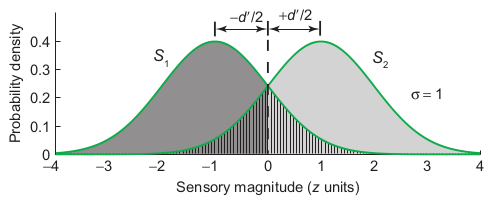
\includegraphics[scale=0.7]{../imagenes/modelosthurst.png}
			    \centering
			    \caption{Ejemplo de cálculo de d' utilizando modelos thursthonianos. Fte: \cite{PsychophysicsB} }
			    \label{fig:modelost}
            \end{figure}
            
            Además de lo ya expuesto, este tipo de análisis es especialmente interesante porque nos permite ordenar los valores obtenidos para $d'$ de forma que las diferencias entre ellos nos da información cuantitativa sobre cómo de diferentes o de similares son cada una de las distribuciones. Con la facilidad añadida que tiene este sistema para representar gráficamente mediante las técnicas habituales como diagramas de barras, entre otros.
    
    
    \bibliography{biblio}
    \bibliographystyle{ieeetr}
\end{document}